%----------
%   WARNING
%----------

% This Guide contains Library recommendations based mainly on APA and IEEE styles, but you must always follow the guidelines of your TFG Tutor and the TFG regulations for your degree.

% THIS TEMPLATE IS BASED ON THE IEEE STYLE 


%----------
% DOCUMENT SETTINGS
%----------

\documentclass[12pt]{report} % font: 12pt

% margins: 2.5 cm top and bottom; 3 cm left and right
\usepackage[
a4paper,
vmargin=2.5cm,
hmargin=3cm
]{geometry}

% Paragraph Spacing and Line Spacing: Narrow (6 pt / 1.15 spacing) or Moderate (6 pt / 1.5 spacing)
\renewcommand{\baselinestretch}{1.15}
\parskip=6pt

% Color settings for cover and code listings 
\usepackage[table]{xcolor}
\definecolor{azulUC3M}{RGB}{0,0,102}
\definecolor{gray97}{gray}{.97}
\definecolor{gray75}{gray}{.75}
\definecolor{gray45}{gray}{.45}

% PDF/A -- Important for its inclusion in e-Archive. PDF/A is the optimal format for preservation and for the generation of metadata: http://uc3m.libguides.com/ld.php?content_id=31389625. 

% In the template we include the file OUTPUT.XMPDATA. You can download that file and include the metadata that will be incorporated into the PDF file when you compile the memoria.tex file. Then upload it back to your project.  
\usepackage[a-1b]{pdfx}

% LINKS
\usepackage{hyperref}
\hypersetup{colorlinks=true,
	citecolor=black,
	linkcolor=black, % links to parts of the document (e.g. index) in black
	urlcolor=blue} % links to resources outside the document in blue

% MATH EXPRESSIONS
\usepackage{amsmath,amssymb,amsfonts,amsthm}

% Character encoding
\usepackage{txfonts} 
\usepackage[T1]{fontenc}
\usepackage[utf8]{inputenc}

% English settings
\usepackage[english]{babel} 
\usepackage[babel, english=american]{csquotes}
\AtBeginEnvironment{quote}{\small}

% Footer settings
\usepackage{fancyhdr}
\pagestyle{fancy}
\fancyhf{}
\renewcommand{\headrulewidth}{0pt}
\rfoot{\thepage}
\fancypagestyle{plain}{\pagestyle{fancy}}

% DESIGN OF THE TITLES of the parts of the work (chapters and epigraphs or sub-chapters)
\usepackage{titlesec}
\usepackage{titletoc}
\titleformat{\chapter}[block]
{\large\bfseries\filcenter}
{\thechapter.}
{5pt}
{\MakeUppercase}
{}
\titlespacing{\chapter}{0pt}{0pt}{*3}
\titlecontents{chapter}
[0pt]                                               
{}
{\contentsmargin{0pt}\thecontentslabel.\enspace\uppercase}
{\contentsmargin{0pt}\uppercase}                        
{\titlerule*[.7pc]{.}\contentspage}                 

\titleformat{\section}
{\bfseries}
{\thesection.}
{5pt}
{}
\titlecontents{section}
[5pt]                                               
{}
{\contentsmargin{0pt}\thecontentslabel.\enspace}
{\contentsmargin{0pt}}
{\titlerule*[.7pc]{.}\contentspage}

\titleformat{\subsection}
{\normalsize\bfseries}
{\thesubsection.}
{5pt}
{}
\titlecontents{subsection}
[10pt]                                               
{}
{\contentsmargin{0pt}                          
	\thecontentslabel.\enspace}
{\contentsmargin{0pt}}                        
{\titlerule*[.7pc]{.}\contentspage}  


% Tables and figures settings
\usepackage{multirow} % combine cells 
\usepackage{caption} % customize the title of tables and figures
\usepackage{floatrow} % we use this package and its \ ttabbox and \ ffigbox macros to align the table and figure names according to the defined style.
\usepackage{array} % with this package we can define in the following line a new type of column for tables: custom width and centered content
\newcolumntype{P}[1]{>{\centering\arraybackslash}p{#1}}
\DeclareCaptionFormat{upper}{#1#2\uppercase{#3}\par}
\usepackage{graphicx}

% CODE LISTINGS
% support and styling for listings. More information in  https://es.wikibooks.org/wiki/Manual_de_LaTeX/Listados_de_código/Listados_con_listings
\usepackage{listings}

% Custom listing
\lstdefinestyle{estilo}{ frame=Ltb,
	framerule=0pt,
	aboveskip=0.5cm,
	framextopmargin=3pt,
	framexbottommargin=3pt,
	framexleftmargin=0.4cm,
	framesep=0pt,
	rulesep=.4pt,
	backgroundcolor=\color{gray97},
	rulesepcolor=\color{black},
	%
	basicstyle=\ttfamily\footnotesize,
	keywordstyle=\bfseries,
	stringstyle=\ttfamily,
	showstringspaces = false,
	commentstyle=\color{gray45},     
	%
	numbers=left,
	numbersep=15pt,
	numberstyle=\tiny,
	numberfirstline = false,
	breaklines=true,
	xleftmargin=\parindent
}

\captionsetup*[lstlisting]{font=small, labelsep=period}
 
\lstset{style=estilo}
\renewcommand{\lstlistingname}{\uppercase{Código}}


% REFERENCES 

%-------------
%	DOCUMENT
%-------------

\begin{document}
\pagenumbering{roman} % Roman numerals are used in the numbering of the pages preceding the body of the work.

%----------
%	COVER
%----------	
\begin{titlepage}
	\begin{sffamily}
		\color{azulUC3M}
		\begin{center}
			\begin{figure}[H] % UC3M Logo
				\makebox[\textwidth][c]{
\includegraphics[width=10cm]{Figures/template/UWTSD-Logo.png}}
			\end{figure}
			\vspace{2.5cm}
			\begin{Large}
				MSc Degree in Software Engineering and Artificial Intelligence\\
				2022-2023\\ % Academic year
				\vspace{2cm}
				\textsl{MSc Thesis}
				\bigskip

			\end{Large}
			{\Huge ``Enhancing Self-Driving Car Performance: The Potential Dangers of Autonomous Vehicles and Motorcycles''}\\
			\vspace*{0.5cm}
			\rule{10.5cm}{0.1mm}\\
			\vspace*{0.9cm}
			{\LARGE Edward Samuel Ralph Patch}\\
			\vspace*{1cm}
			\begin{Large}
				Dr. Tim Bashford\\
				Waterfront Campus - 2023\\
			\end{Large}
		\end{center}
		\vfill
		\color{black}

	\end{sffamily}
\end{titlepage}

\newpage % blank page
\thispagestyle{empty}
\mbox{}

\newpage % blank page
\thispagestyle{empty}
\mbox{}

%----------
%	ABSTRACT AND KEYWORDS 
%----------	
\renewcommand\abstractname{\large\bfseries\filcenter\uppercase{Summary}}
\begin{abstract}
	\thispagestyle{plain}
	\setcounter{page}{3}

	% Write your abstract
	Abstract

	\textbf{Keywords:} % add the keywords
	Artificial Neural Networks, Autonomous Vehicles, Motorcycle Safety.
	\vfill
\end{abstract}
\newpage % Blank page
\thispagestyle{empty}
\mbox{}
%----------
%	Acknowledgements
%----------	
\chapter*{Acknowledgements}
	We extend our deepest gratitude to Kaden Summers and Jonathon Patch, whose invaluable contributions as motorcyclists greatly enriched this project. Their tireless efforts in capturing testing footage from Carmarthenshire to Powys in Wales, under rainy and clear conditions provided critical qualitative data to our research. The visual material they obtained was instrumental in offering a comprehensive understanding of the subject.
	
	Special appreciation goes to Jonathon Patch, who participated in the fieldwork and generously provided the camera equipment necessary to record the footage. Their collaboration and unwavering support have played a pivotal role in advancing this research; for that, we are profoundly thankful.

\setcounter{page}{5}

% Write here	
\vfill

\newpage % blank page
\thispagestyle{empty}
\mbox{}


%----------
%	TOC
%----------	

%--
% TOC
%-
\tableofcontents
\thispagestyle{fancy}

\newpage % blank page
\thispagestyle{empty}
\mbox{}

%--
% List of figures. If they are not included, comment the following lines
%-
\listoffigures
\thispagestyle{fancy}

\newpage % blank page
\thispagestyle{empty}
\mbox{}

%--
% List of tables. If they are not included, comment the following lines
%-
\listoftables
\thispagestyle{fancy}

\newpage % blankpage
\thispagestyle{empty}
\mbox{}


%----------
%	THESIS
%----------	
\clearpage
\pagenumbering{arabic} % numbering with Arabic numerals for the rest of the document.	

\chapter{Introduction}

\chapter{Project Objectives}
\label{chap:projectObjectives}
	% REREAD through each section and adjust accordingly.
	
	The project involves the research, design, experimentations and findings to answer the research question. The hypothesis statements will drive the development of the study and investigations to provide a statistical analysis of any potential safety issues.

	\section{Research Hypothesis}
		This paper will cover blindspots and poor weather conditions hypothesis statements. The following hypothesis statements are orientated for the dissertation paper exploring the research question, `Are AVs a Danger to Motorcyclists?':

		\begin{enumerate}
			\item Motorcycles have blindspots that are often overlooked by human drivers, which AVs can detect and avoid.
			\item In low light conditions, AVs may struggle to accurately detect and identify motorcycles, leading to potential safety issues on the road.
			\item Poor weather conditions, such as heavy rain or poor visibility, can make it difficult for AVs to detect and react to motorcycles, increasing the risk of accidents.
		\end{enumerate}

	\section{Outline}
        The study will select relevant Machine Learning/Deep Learning (ML/DL) models, hyper-parameters and techniques, with some existing research to support the experimentation results. Some initial research papers and datasets are enclosed in this paper. However, if any new research developments are established during the experimentation, then consideration of the research would include in the research section that backs up the investigation. The study will uncover and cover some of the existing research. However, expand on any technicalities to help prove the established hypothesis statements.

	\section{Aim and Objectives}
        The aim of the study is to address the problems with AVs to fulfill the research gap. The problems have been addressed within conference papers and even when it comes to object classifications. Although, with the lowest of incidents, whether it is due to the safety training of motorcyclists or population that actually ride, dependent on the country, the problem is rarely addressed thoroughly. If AVs roll out into regions like Southeast Asia: Indonesia, Vietnam, Thailand and others, and European countries: Italy, Spain, Brazil and others, then the problem will appear more, not allowing organisations to brush the problem `under the rug'. The objective is to find some theoretical logic of the underlying problems and potential solutions or considerations for ADAS/AVs to adapt decreasing any potential tragic accidents.

		The main objectives of this project are to develop an accurate UK Motorcycle trained model using Ultralytic's YOLOv5 architecture and to improve the model's performance on specific tasks. The following steps will support the experimentation to answer the research questions:

        \begin{enumerate}
            \item \textbf{Dataset Preparation:} Object Classification requires a set of labels to correspond to an image, mapping different classified objects within the image. Preparation of the data requires being able to select validated data for training and testing purposes.
            \item \textbf{Pre-processing:} Read in the mapping datasets and extract the sorted datasets to the designated file paths. 
            \item \textbf{Architecture Selection and Optimisation:} Investigate different object classification architectures, and select a model that could closely demonstrate an idea of how AVs currently initialise object classification.
            \item \textbf{Evaluation Techniques:} Confusion Matrix and PR-Curve are tools to fine-tune and evaluate the model's training performance.
        \end{enumerate}

	\section{Project Structure}
        The research during the project must justify tools to support image preprocessing, analysing and classification to provide an understanding of the problems taking place. Image preprocessing is a significant consideration in the project to answer all the hypotheses, as motorcycles may be in a blind spot, but with better adjustments, the image classification could see blur or shadows easier with sharper settings or if the time and weather have poor visibility, then dangerous the image to greyscale, and increasing edge sharpness could help make the motorcycle outline more clear. Different classification methods can improve the accuracy of a data model, including using various layers, hyper-parameters, and techniques during the training of a dataset.

        The experiment would look into image classification with the selected dataset providing information on possible misclassifications from the chosen dataset. The image classification structure would follow some standards that AVs use. However, AVs would use object classification libraries that support real-time footage. Image classification aims to see how motorcycles are identified among other vehicles to extend the research.

        Some of the strategies to determine the hypothesis statements is to select a model like DBN and CNN or R-CNN and to compare the results with the corresponding research results. Find image classification research papers for example, `An Analysis of Convolutional Neural Networks For Image Classification' researched by Neha Sharma~\cite{sharma_analysis_2018} demonstrates a good example of a CNN structure. 

        This AI project will involve seven phases in accordance with the paper `Developing ML/DL Models: A Design Framework' authored by Meenu Mary John~\cite{john_developing_2020} involving Business Case Specification, Data Exploration, Feature Engineering, Experimentation, Development, Deployment and Operational. The Business Case Specification, in this case, is to find out if motorcycles are in danger around AVs and find suggestions or research pathways to answer the hypothesis that supports the research question thoroughly. It is essential to find datasets that support the business case specifications. During the data exploration phase, exploring some available datasets and filtering them out to better back the research question is essential. 
        
        Feature engineering takes place to determine the relevant data fields or features that benefit the study. For example, non-vehicle objects like traffic lights and pedestrians are not required if the focus is on motorcycles. Although, it can be equally argued that when AVs function, they process many objects simultaneously for better awareness. 
      
        The experimentation phase includes developing a model for the dataset, compiling the model and reviewing the data to optimise the model for the dataset. This experimentation will already shape potential issues with the dataset. Each time the data is run with different tunings, it will help develop an idea of the potential issues with the dataset. 
      
        The development phase is where findings from the experimentation are presented. This phase will formalise the results and suggest to the target audience the project's future work. 
      
        The Deployment and Operational phases are not required. However, a replacement of a Review phase may be where results and findings can be discussed, and any suggestions to optimise the experimentations for future work.

	\section{Sourcing and Preparation}
		The datasets being used are arranged in YOLOv7 format and would require additional modifications to work before the training phase. The datasets that have been decided to train the models are `Motorcycle Samples - v1 VMT-V1', sourced from Roboflow~\cite{roboflow_motorcycle_nodate}, and `Road Vehicle Images Dataset', sourced from Kaggle, authored by Ashfak Yeafi~\cite{ashfak_yeafi_road_nodate}.

		The training materials are split into `images' and `labels' categories, which require some preparation. Using Python scripts, the selected training material is taken and processed together, allowing the model to see different motorcycles in different scenarios. A US and Indian dataset was used to get other road conditions and various types of motorcycles. Using the two datasets should help increase the accuracy during the training and validation process. The materials are separated and combined into a CSV file format, and another Python Snippet can reconstruct the CSV and Image Data into a new directory.

	\section{Pre-Processing}
		Training of two datasets, dataset A with the filter of `bus', `car', `minivan', `motorcycle', `pickup', `scooter', `trike', `truck', `van', `person', whereas dataset B involves; `motorcycle', `tricycle' and `person' filters. The `yolov5s.pts' and `yolov5l.pts' were used during testing, with better results on the `yolov5l.pts' by 25\% when identifying motorcycles. Both weights used a batch of thirty-two and ten epochs.

		Testing materials must include video content, split into multiple frames to test the trained YOLO model, with enough images to create a strong argument. Joining a motorcycle group and exploring various routes across the United Kingdom, including motorways, dual carriageways, A-roads, and backroads, with motorcycles overtaking, filtering, and navigating blindspots, can lead to unexplored scenarios and questions that may have been previously overlooked.
					
		A decided factor is to use a Drift Innovation Ghost XL motorcycle camera attached to a motorcycle that rides within the group, then swap the camera with another rider after some time. This way, combining the content helps identify how Object Classification copes with numerous blindspots and draws some questions to further the research concerning the current safety of AV vehicles. 
		
		One sports bike and two cruisers are selected for material to test how Object Classification models handle different motorcycle styles. Ideal footage would include Scramblers, Trikes and other similar vehicles to establish how Object Classification models work in an estimated manner. A perfect material would be that during the ride out, conducted on 18$^\text{th}$ July 2023, Tuesday, would capture these vehicles, which either pass by or join us in sections of the rides. The group is instructed to overtake and be undertaken by the camera vehicle to create plenty of footage to put the YOLO model to the test.

	\section{Evaluation Metrics}
        During the experimentation, it is necessary to discuss of how the analyst of experimental data may take place. This information will guide the project with relevant data backing up the optimisation and accuracy during the ML prototyping, and gathering feedback for the research question to present the findings and develop any potential solutions or future work.

        Two common methods of observing performance and accuracy among the different classes available within a dataset is Confusion Matrices and Classification Reports. These tools provide a clear indication of overfiting, underfitting and accuracy. The confusion matrix does this by demonstrating true positives and false positives, which the main focus to back up the research question would be the Motocycle feature to see where any false positives are detected. The Classification Report displays a range of information involving `Precision', `Recall', `F1-Score' and `Support' of each features; detailing any potential issues of outliers. Three averages: `Accuracy', `Macro Avg' and `Weighted Avg.' are included to show the overall accuracy of the model.~\cite{liang_confusion_2022}~\cite{panigrahi_deep_2018}

        As Neural Networks train with a given epoch, meaning how many iterations the test data would go through training. A history of these iterations will be on record and displayed on a `Validation and Training Loss' graph to indicate the loss gap of the initial learning and the fitness of the trained and validation data to indicate the performance and any potential improvements,~\cite{panigrahi_deep_2018}

\chapter{Literature Review}
\label{chap:literatureReview}
	\section{Autonomous Vehicle Paradigm and Legalities}
		Firstly, it is essential to understand how vision works on AV and what techniques are in place to allow vehicles to function correctly and safely. Journal Article, `AVs: from paradigms to technology', authored by Silviu Ionita~\cite{ionita_autonomous_2017}, offers underlying information about the foundation of autonomous vehicle systems. It is equally important to understand how motorcycles function within traffic and the reasoning behind motorcyclist mentality.

		Motorcycling filtering laws vary in different countries globally. Australia and USA states have different definitions of filtering. Some states declare filtering legal, whereas other states declare filtering illegal. Thailand country made filtering illegal. However, some of these states or countries where filtering is illegal are poorly policed, indicating that motorcyclists may filter if an opportunity arises. That means AV vehicles should anticipate filtering even in countries/states where filtering is illegal to minimize the number of casualties and incidents.~\cite{promraksa_lane-filtering_2022}

		An `intelligent vehicles' paradigm has three logical rule statements to follow. Firstly, the system will collect data from the driver, developing the knowledge from itself and the driver. Second, the system will have to perform some judgement. Silviu Ionita~\cite{ionita_autonomous_2017} mentions that it is paramount to filter the data through logical statements and apply multivalent logic to handle uncertainty better, creating a better judgement. ADAS require consistent autonomous behaviour to collect and handle the data even when the system is not in control. This behaviour means that the developers can collect data on what the system would have done if it were in control, allowing any refinement down the line and enabling AVs to work more efficiently.

		Figure~\ref{fig:adasFunctionsIonita} provides the structure of Advanced Driver Assistance Systems (ADAS) functions linking the responsibilities to the decision and action. Strategic Processes are near real-time, Tactical Processes are real-time, and Direct Processes are short as possible. These three functionalities are fundamental when understanding how an ADAS vehicle copes and how an AV will tend to handle situations.~\cite{ionita_autonomous_2017} It is necessary to establish that the AV will only rely on its judgement after the decision to remove human interaction. Some of these system paradigms reflect the capabilities of AVs involving blindspots, low-light and poor weather conditions.
		\begin{figure}[h]
			\centering
			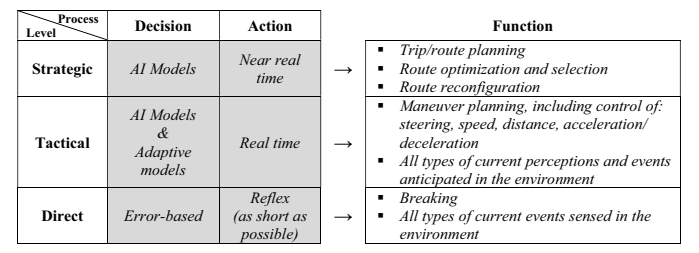
\includegraphics[width=\columnwidth]{Figures/literature_review/proposal/SystemFunctionality-3.png}
			\caption{Classes of ADAS and their Requirements for Decision and Execution~\cite{ionita_autonomous_2017}}
			\label{fig:adasFunctionsIonita}
		\end{figure}

	\subsection{Vision Technology and Techniques}
		When investigating how AVs handle blindspot handling compared to human drivers, the paper `Automated driving: Safety blind spots' by Ian Y. Noy~\cite{noy_automated_2018} suggests the current implementations within ADAS and compares it to standard driving errors. Although, the paper does not directly reflect on motorcycles, the paper details ADAS systems and how the transition from ADAS to AVs is possible. An important quote from the paper is that `AD technologies are suboptimal in that they fail to address critical blind spots and will likely lead to unnecessary losses and injuries because insufficient consideration is given to integrating the human element into overall sociotechnical road transportation system'~\cite{noy_automated_2018} suggests that transitioning from ADAS to AVs is relatively dangerous if blindspot judgements are overlooked. With further research in this area, it will provide more information to understand if AVs are safer than human drivers on the road.

		Light Detection and Ranging (LiDAR) uses a pulsed laser to gather information about the object surroundings, providing depth that images cannot capture. Within the paper, `Pedestrian recognition and tracking using 3D LiDAR for autonomous vehicle' by Heng Wang~\cite{wang_pedestrian_2017}, a quote ``LiDARs are another kind of commonly used sensors for pedestrian recognition, compared with cameras, LiDARs can provide accurate range information and larger field of view.''. Heng Wang points out that the use of LiDAR widens the field of view.
		
		After researching some extra information, it was found within the report `What Happens for a ToF LiDAR in Fog?'~\cite{li_what_2021} that the failure rate of detection in Diffuse Reflection Targets: 2.1\% and Retro-Reflective Objects: 0.7\% in the range of 0-10m, Diffuse Reflection Targets: 10.3\% and Retro-Reflective Objects: 1.1\% in the range of 10-15m, Diffuse Reflection Targets: 15.1\% and Retro-Reflective Objects: 1.1\% in the range of 15-20m, and Diffuse Reflection Targets: 19.5\% and Retro-Reflective Objects: 0.7\% in the range of 0-10m~\cite{royo_overview_2019}

		When investigating how AVs handle blindspot handling compared to human drivers, the paper `Automated driving: Safety blind spots' by Ian Y. Noy~\cite{noy_automated_2018} suggests the current implementations within ADAS and compares it to standard driving errors. Although the paper does not directly reflect on motorcycles, the paper details ADAS systems and how the transition from ADAS to AVs is possible. An important quote from the paper is that `AD technologies are suboptimal in that they fail to address critical blind spots and will likely lead to unnecessary losses and injuries because insufficient consideration is given to integrating the human element into overall sociotechnical road transportation system'~\cite{noy_automated_2018} suggests that transitioning from ADAS to AVs is relatively dangerous if blindspot judgements are overlooked. Further research in this area will provide more information to understand if AVs are safer than human drivers on the road.

	\section{Model Architectures}
		Yen-Yi Wu~\cite{wu_pedestrian_2016} suggests using a Deep Belief Networks (DBN) model for object classification. The model correctly classifies images: pedestrians, bikes, motorcycles and other vehicles. The model thrives an 89.53\% accuracy.

		The r-CNN model merges a CNN approached model with a Region-based model to create a deeper layered one. The aim is to increase accuracy and performance regarding object classification. The R-CNN uses a selective search algorithm to find certain features within the set of images and focus on the objects that match the specified features using diverse strategies. This approach means that when training the model, it is equally important to understand what the layers do and how they filter the image to change the test data to analyse the different performances and accuracies of the training and testing.~\cite{uijlings_selective_2013}~\cite{ren_faster_2015}

		DBN model is based on Restricted Boltzmann Machine (RBM) layers to train the model. According to `An overview on Restricted Boltzmann Machines'~\cite{zhang_overview_2018} explains that RBMs pre-train the networks' weights. This technique is done layer by layer and applies gradient descent methods to fine-tune the weights. This method alone allows the neural network to optimise the hyper-parameters, which in turn boosts accuracy and optimises the model's overall performance.

		Both model suggestions both use CNN, whether it is merging CNN or comparing to CNN. The Journal Article titled "Detection of Motorcyclists without Helmet in Videos using Convolutional Neural Network" by C. Vishnu includes a layer designed to recognise whether a motorcyclist is wearing a helmet. This finding emphasises an essential feature in ensuring the safety of riders on the road. Using a Convolutional Neural Network, the layer can accurately detect whether a helmet is being worn, which can help prevent accidents and reduce injuries. It is impressive to see how technology can enhance safety measures in everyday life. The layers proposed by the author should benefit the datasets used in this research project. The layer structure is fatigue, although it involves ReLU, max-pooling, fully connected and a loss function (Support Vector Machines or Softmax) layers.
        
        Figure~\ref{fig:adasFunctionsIonita} displays the DBN and RBM layers from the paper, `Parallel computing method of deep belief networks and its application to traffic flow prediction' illustrated by Lu Zhao~\cite{zhao_parallel_2019}. DBN is not a convolutional network compared to CNN. DBN consists of a two-layer graph, including a visible layer below and a hidden layer above, displayed in figure~\ref{fig:dbnRBMLayers}. The author and illustrator mention that the RBM layers illustrated are slightly different to the classical Boltzmann Machine.~\cite{zhao_parallel_2019}

		\begin{figure}[htp]
			\centering
			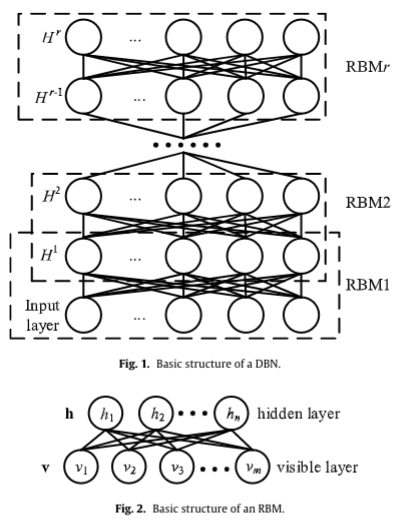
\includegraphics[width=\columnwidth]{Figures/literature_review/proposal/DBNRBMLayers.png}
			\caption{DBN and RBM Model Layers~\cite{zhao_parallel_2019}}
			\label{fig:dbnRBMLayers}
		\end{figure}

	\section{Datasets and Preparation Idealogies}
		Finding the suitable dataset for the given research question involves first identifying the required information. The requirements of the dataset need to have motorcycles on the road with different situations, camera angles and visibility. After exploring through some datasets, three image classification datasets, `TuSimple'~\cite{jeong_end--end_2017}, `Car vs Bike Classification'~\cite{deepnets_car_nodate} and `MB10000'~\cite{espinosa_motorcycle_2018}. The ideal datasets at the time was `TuSimple'. However, the dataset was twenty-five gigabytes, and meant that training the dataset was too much for individual research. The `Car vs Bike Classification' dataset lacked authentic motorcycle and car images in realistic situations. However, the dataset was lightweight, with one hundred and eight megabytes. These mentioned specifications meant that the `MB10000' had an optimistic fitness to support this experiment. The dataset has realistic situations, motorcycles with other vehicles and image sequences to support image classification. The dataset has four-hundred and twenty-six megabytes of filesize.

		`Pedestrian, Bike, Motorcycle and Vehicle Classification via Deep Learning: Deep Belief Network and Small Training Set' by Yen-Yi Wu~\cite{wu_pedestrian_2016} goes over different visibility levels that affect pedestrians, bikes, motorcycles and vehicles and how image classification affects these vehicles. The image preprocessing involves converting colour images to greyscale. Including edge emphasis, detection to enhance to the image, with the fundamental aim to detect edges of objects seamlessly. The paper suggests using a fixed threshold and Otsu methods to threshold greyscale images and use bilinear interpolation for image resizing. These methods should increase the visibility of the objects within the images are good notes for when conducting any experiments.

\chapter{Research Methodology}
\label{chap:researchMethodology}
	\section{Fundamental Research}
		Fundamental research methodology builds a directive of a research area driven by curiousity. This type of research collection increases the understanding of a selected research topic, which is vital in cases where not many research papers exist. Fundamental research papers alone are not substantial to start developing towards a research project, as the name suggests, it creates a foundation and provides insights to understanding any problems found during the research study. These papers tend to cover basic understandings of phenomenon's, which in turn backs up the research question. These research materials may include surveys, interviews, observations and experiments.~\cite{saunders_research_2012}

		In the context of AVs and motorcycles, the research methodology seeks to understand any underlying principles of the interaction of these vehicle types on the road. It may even contain discussions and analytics of crash data or theoretical requirements that AV organisations should follow. For example, a study of how drivers and rider perceive each other on the road would impact the research approach, taking in account of the AVs visibility requirements. For the project, consideration of conference papers, case studies and surveys should help form any research directives to approach the testing of the hypotheses statements.

	\section{Statistical Research}
		Statistical research is a critical component of this research project, as interpreting the analytical data generated from the Neural Network is important. AVs and ADAS are complex systems, and require a good understanding of the statistics of real life events to understand hypothetical situations. The goal of statistical research is to identify patterns, relationships and trends within the data. These three variables allow the testing about each individual hypothesis and forming the conclusions of the research method.

		Statistical research could involve comparing other object classifications papers involved with AVs and motorcycles, taking account of the design plan, neural network model and layers, results and discussions to give an understanding of industry standard results. This also gives a great way to test the findings from the research project against the statistical findings and then form a detailed report of the findings, and provide a useful further work section. Statistical research has been demonstrated to make sure that the datasets are relevant and up-to-date Use Cases, and to understand the initial problems with motorcycles and ADAS/AVs to develop the research question.

	\section{Quantitative Research}
		Quantitative research involves the numerical data to collect and analyse data. This has a secondary importance similarly to the fundamental research methodology. This research collection appears a few times whether it is working with the algorithm, Confusion Matrix or understanding numerical data gathered from fundamental and statistical research papers to understand of variables in relation of AVs and motorcycles. Quantitative research methodology can help with identifying and aids with developing evidence-based recommendations for improving motorcycle safety.

		Quantitative research methodology tends to involve surveys, questionnaires and user studies. The methods enable the research to contain a large amounts of numerical data related to the research question. Numerical techniques can also provide tools to conduct correlation analysis and hypothesis testing, in accordance with research from the statistical side and experimental results. The quantitative methods has been applied to check performance, size and other key factors when it comes to preparing the Neural Network to make sure that the hypotheses are accurate and workable.

	\section{Qualitative Research}
		Qualitative research is a crucial factor of this project. As seen in this proposal, datasets had to be observed to make sure they could withstand the hypotheses. During the prototyping and evaluating of the model, observations will be made and cross-referenced to make sure that the findings are accurate. This type of testing could help work out any potential issues with current data structures or even provide some awareness of problems that may have not been considered before. It is also important to make notes from other research projects with qualitative research to consider any key points.

		In addition, observation studies could help enhance the research development. This could be finding case studies that provide videos of AVs in process with descriptions of what the program is doing and what systems are in place. This content could involve indepth interviews with experts and stakeholders to understand AVs and motorcycle's current interactions and known concerns. It could also be a useful tool communicating to some motorcycle instructors or experts to understand if there is any on-going issues with ADAS vehicles and motorcycles. These could aid the study further in seeing or hearing the experiences.

\chapter{Development Methodology}
\label{chap:developmentMethodology}
	Due to the nature of the AI project, the Agile development methodology does not fit. Although, if the project involves a team of developers, then the Agile development methodology will make the better fit. The AI project has a small team and requires a lot of repetition to find the best fit and results for the experimentation. The Iterative development methodology is the best approach. The Agile Methodology could cost anywhere from £422.91 (Freelancer Team Members) to £2085.04 (Payroll Team Members)~\cite{owais_effort_2016} 
	
	Where usually, Agile development methodology has an initial cost factor, and the development saves coordination, flexibility and performance within a team development environment. However, it does not fit in a project that aims to deliver results to address a safety issue. The Agile methodologies, Iterative and Rapid Application Development (RAD) development methodologies address this project better, with the ability to make a prototype model, test and refine it. 

	RAD is a risky methodology as it does not allow the flexibility to redesign the plans to enable definition when addressing the given safety concern. Therefore, the Iteration development model is an ideal solution, allowing the ability of initial planning and then additional planning and requirement changes, also continuously updating the analysis and design, testing and evaluation. This key methodology cycle will benefit the ideology of setting the layers up and evaluating the results. Agile Methodology also uses User Stories, which is excellent if a platform is being made. However, the user stories would get repetitive during the research project, which wastes time in this specific scenario.

	\section{Iterative Development Methodology}

\chapter{Reflection}

\chapter*{Terminology}
List of terminologies used in this document:-
\begin{itemize}
	\item AV - Autonomous Vehicles.
\end{itemize}

%----------
%	Bibliography
%----------	

\clearpage
\nocite{*}
\small{\bibliographystyle{IEEEtran}
	\bibliography{ref}}

%----------
%	Appendix
%----------	

% If your work includes Appendix, you can uncomment the following lines
%\chapter* {Appendix x}
%\pagenumbering{gobble} % Appendix pages are not numbered

\end{document}